\chapter{Contributions to NP optimization problems}
\label{chap:softagents}

The chapter begins with a short overview of NP completeness and NP optimization problems in Section \ref{sec:np}. The rest of the chapter is entirely original and presents our contribution to NP optimization problems, focusing on two  well-known NP-hard problems: Travelling Salesman Problem (TSP) and Set Covering Problem (SCP).

The approaches presented in this chapter represent original works published in \cite{Chira07Stigmergic, Gaceanu12SCP}.

The chapter is structured as follows. In Section \ref{sec:np} a short overview of NP completeness is made. In Section \ref{sec:stigmergic} the travelling salesman problem is approached using the stigmergic agent model. The Stigmergic Agent System (SAS) combines the strengths of Multi-agent Systems (MAS) and Ant Colony Systems (ACS).  Stigmergy provides a general mechanism that relates individual and colony level behaviours: individual behaviour modifies the environment, which in turn modifies the behaviour of other individuals. The stigmergic agent mechanism employs several agents able to interoperate in order to solve problems by using both direct communication and indirect (stigmergic) communication. The algorithm was evaluated on several standard datasets outlining the potential of the method. 
In Section \ref{sec:softagents} the soft agent model is introduced. A soft agent is an intelligent agent that has to deal with imprecision, uncertainty, partial truth and approximation during its execution as a reactive agent or goal oriented agent or both. This new agent model is used in Section \ref{sec:scp} where a new incremental clustering approach to the Set Covering Problem is presented. Experiments on standard datasets suggest that the approach is promising. Section \ref{sec:scpconcfw} outlines the conclusions of the chapter and indicates future research directions.

The original contributions of this chapter are:

\begin{itemize}
\item A stigmergic agent system algorithm for solving the travelling salesman problem (Section \ref{sec:stigmergic}) \cite{Chira07Stigmergic}.
\item A new model for software agents: the soft agent model (Section \ref{sec:softagents}) \cite{Gaceanu12SCP}.
\item An incremental clustering algorithm for solving the set covering problem (Section \ref{sec:scp}) \cite{Gaceanu12SCP}.
\item Experimental evaluation of both algorithms on standard datasets (Section \ref{sec:stigmergic} and Section \ref{sec:scp}) \cite{Chira07Stigmergic, Gaceanu12SCP}.
\end{itemize}




\section{NP-completeness}
\label{sec:np}

Problems for which the required  time for solving a problem from this class using any nowadays available algorithm increases very fast as the problem size grows are called NP-complete.
Nevertheless it is still necessary to somehow deal with these problems. In many situations approximation algorithms are used in order to address NP-complete problems \cite{Cormen09Introduction}.



\begin{definition}
\label{def:npc}
A decision problem $L$ is called NP-complete if:
\begin{enumerate}
\item $L \in NP$ and
\item $L^{'} \leq p~L, \forall L^{'} \in NP$,
\end{enumerate}
where $L^{'} \leq p~L$ means that $L^{'}$ is reducible to $L$ in polynomial time.
\end{definition}

\begin{definition}
A problem is NP-hard if it satisfies only the second property from Definition \ref{def:npc} and not necessarily the first one.
\end{definition}

Perhaps the most interesting aspect of NP-completeness is the property that if a single NP-complete problem can be solved in polynomial time then there an algorithm solvable in  polynomial time for all NP-complete problems, i.e., $P=NP$ (where $P$ is the class of problems solvable in polynomial time and $NP$ is the class of problems solvable  in nondeterministic polynomial time). The $P \neq NP$ is the most interesting open problems in the theory of computer science \cite{Cormen09Introduction}.

There are many examples of NP optimization problems \cite{compediumnp} and we will discuss about two of them in the next sections, namely the Travelling Salesman Problem (TSP) and The Set Covering Problem (SCP).


\section{Stigmergic agents}
\label{sec:stigmergic}

In \cite{Chira07Stigmergic} a Stigmergic Agent System (SAS) combining the strengths of Ant Colony Systems and Multi-Agent Systems concepts is proposed. The agents from the SAS are using both direct and indirect (stigmergic) communication. 
Stigmergy occurs as a result of individuals interacting with and changing an environment \cite{Dorigo04Ant}. Stigmergy was originally discovered and named in 1959 by Grasse, a French biologist studying ants and termites. Grasse was intrigued by the idea that these simple creatures were able to build such complex structures. The ants are not directly communicating with each other and have no plans, organization or control built into their brains or genes. Nevertheless, ants lay pheromones during pursuits for food, thus changing the environment. Even though ants are not able to directly communicate with each other, they do communicate however --- indirectly --- through pheromones.

Stigmergy provides a general mechanism that relates individual and colony level behaviours: individual behaviour modifies the environment, which in turn modifies the behaviour of other individuals.

The SAS mechanism employs several agents able to interoperate on the following two levels in order to solve problems:
\begin{itemize}
\item
	direct communication: agents are able to exchange different types of messages for  knowledge sharing  and  direct interoperation support; the knowledge exchanged refers to both local and global information
\item
	indirect (stigmergic) communication: agents have the ability to produce pheromone trails that influence future decisions of other agents within the system.
\end{itemize}

The initial population of active agents has no knowledge of the environment characteristics. Each path followed by an agent is associated with a possible solution for a given problem. Each agent leaves pheromone trails along the followed path and is able to communicate to the other agents of the system the knowledge it has about the environment after a complete path is created.By using direct communication the risk of getting trapped in local optima is lower. In order to better express the idea, the Stigmergic Agent System (SAS) algorithm for solving the Travelling Salesman Problem (TSP) from \cite{Chira07Stigmergic} is given in Algorithm \ref{alg:sastsp}.

\begin{algorithm}
\caption{SAS for TSP}
\label{alg:sastsp}
\begin{algorithmic}[1]

\STATE @ initialize noOfAgents, stigmergyLevel, startingCity, knowledge base
\WHILE {true} 
	\STATE LaunchAgents (noOfAgents, stigmergyLevel, startingCity)
	\STATE @ wait until all agents finish execution
	\STATE @ handle best solution found - a global update rule is applied, that is, update the pheromone level and store the best solution found so far
\ENDWHILE

\end{algorithmic}
\end{algorithm}

\begin{algorithm}
\caption{LaunchAgents}
\label{alg:launch}
\begin{algorithmic}[1]

\FOR {i = 0 \TO noOfAgents}
\STATE Agent agent = createAgent(stigmergyLevel, startingCity)
\STATE @  execute the agent's behaviour
\ENDFOR
\end{algorithmic}
\end{algorithm}

\begin{algorithm}
\caption{AgentBehavior}
\label{alg:behaviour}
\begin{algorithmic}[1]

\WHILE {a solution is not found}
	\STATE @ proactively determine if the next city should be chosen stigmergically or using direct communication
	\STATE @ if the agent decides to behave stigmergically then the next city to be visited is chosen using standard 					ACS; otherwise the next city to be visited is chosen using direct communication with the other agents
	\STATE @ handle best solution so far - a local update rule is applied, that is, update the pheromone level
\ENDWHILE

\end{algorithmic}
\end{algorithm}

The Travelling Salesman Problem (TSP) is finding the cheapest round-trip route that visits each city exactly
once and then returns to the starting city, given a list of cities, the cost of moving from one city to another and the starting city. An equivalent formulation in terms of graph theory is: given a complete weighted graph (where the vertices would represent the cities, the edges would represent the roads, and the weights would be the cost or
length of that road), find a Hamiltonian cycle with the least weight \cite{tspgraph99}.

The procedure starts by setting algorithm parameters such as the number of agents, the stigmergy level of the agents, the starting city --- the knowledge base of the system in general. The process runs until certain conditions are met. At the first step agents with the given parameters are launched. Once their task is completed, the best found solution is compared with the best already known solution (if any) and a global update is performed. For updating the pheromone level  the following local update rule (see \cite{cmpintea06}) is used:
    
    \begin{equation}
\tau _{ij}(t+1)=(1-\rho )\tau _{ij}(t)+\rho \frac{1}{n\ast L^{+}},
\end{equation}

where $\tau _{ij}$ represents the stigmergy level of the edge
$(i,j$) at moment $t$,  $\rho $ is the evaporation level and $L^{+}$
is the cost of the best tour.

\qquad The global update rule is similar:

\begin{equation}
\tau _{ij}=(1-\rho )\tau _{ij}(t)+\rho \Delta \tau _{ij}(t),
\end{equation}

where $\Delta \tau _{ij}(t)$ is the inverse cost of the best tour.

Agents are autonomous entities meaning that they can choose
to ignore the path communicated by the system and proactively choose
another city to explore. This is crucial for the SAS success since
only using a purely stigmergic approach the solution of a problem
could be trapped into a local optimum.

The algorithm allows stigmergic selection of the next city based on
the probability (see \cite{cmpintea06}):

\begin{equation}
p_{ij}^{k}=\frac{\tau _{iu}(t)[\eta _{iu}(t)]^{\beta }}{\sum_{o\epsilon J_{i%
}^{k}}\tau _{io}(t)[\eta _{io}(t)]^{\beta }},
\end{equation}

where $J_{i}^{k}$ represents the unvisited neighbours of node $i$ by agent $k$%
, $\eta _{io}(t)$ is \emph{visibility} and denotes the inverse of
the distance from node $i$ to node $o$ and $\beta $ shows what is
more important between the cost of the edge and the pheromone level.

Using direct communication agents can proactively choose another
city to explore. So at a certain point in time if an agent decides
that it should use direct communication it can ask the other agents
if they have already visited a certain city. This way an unexplored
city can be identified and the agent can autonomously choose it as
its next move (regardless of pheromone trail intensities).
Cooperating proactive agents capable of both direct and stigmergic
communication provide a robust way to find a solution greatly
reducing the risk of being trapped into local minima.

SAS algorithm for solving TSP is compared to standard Ant Colony
System (ACS) model. In the ACS algorithm the values of the
parameters were chosen as follows: $\beta$ = 5, $\rho$ = 0.5. 

    Table \ref{tab:sas} presents comparative results of the proposed SAS algorithm and the ACS model for solving some  instances of TSP taken from \cite{tsplib}.


\begin{table}[h]
\label{tab:sas}

  \begin{tabular}{|r|r|r|r|r|r|}
\hline \textbf{Problem} & \textbf{Number of} & \textbf{Number of} & \textbf{Best Known} & \textbf{ACS} & \textbf{SAS}\\
 & \textbf{Agents} & \textbf{Generations} & \textbf{Solution} & \textbf{Result}  & \textbf{Result}\\
\hline
swiss42 & 3 &  30 & 1273 &   1589 &   \textbf{1546}\\
\hline
swiss42 & 5 &  30 & 1273 &   1539 &   \textbf{1517}\\
\hline
swiss42 & 10 &  30 &  1273 &    1491 &    \textbf{1489}\\
\hline
swiss42 & 15 &  30 &  1273 &    1472 &    \textbf{1470}\\
\hline
swiss42 & 20 &  30 &  1273 &    1472  &   \textbf{1439}\\
\hline
bays29 &  3 &   30 &  2020 &    2312 &    \textbf{2312}\\
\hline
bays29 &   5 &    30  &  2020  &    2288  &    \textbf{2225}\\
\hline
bays29 &   10  &  30  &  2020  &    2288  &    \textbf{2209}\\
\hline
bays29  &  15 &   30 &   2020  &    2288  &    \textbf{2202}\\
\hline
bays29 &   20 &   30 &   2020 &     2288  &    \textbf{2177}\\
\hline
gr120  &    3  &    30 &    6942 &      12271 &     \textbf{11999}\\
\hline
gr120  &   5  &   30  &  6942  &    12220  &   \textbf{10339}\\
\hline
gr120  &   10  &  30  &  6942  &    9571  &    \textbf{9548}\\
\hline
gr120  &   15  &  30  &  6942  &    9488  &    \textbf{9488}\\
\hline
gr120  &   20  &  30  &  6942  &    9488  &    \textbf{8668}\\
\hline
\end{tabular}

 \caption{Comparative testing results}
 \label{table:testResults}
 \end{table}

Numerical experiments suggest a beneficial use of direct and
stigmergic communication in cooperative multi-agent systems for
addressing combinatorial optimization problems.





\begin{comment}
\begin{algorithm}
{\small \vspace{2 mm} Stigmergic Agent System}


{\small \hspace{4 mm} Set parameters}

{\small  \hspace{4 mm} Initialize pheromone trails} 

{\small \hspace{4 mm}  Initialize knowledge base}

{\small  \hspace{4 mm} Loop}

{\small  \hspace{8 mm} Activate a set of agents}

{\small   \hspace{8 mm} Each agent is positioned in the search space}

{\small   \hspace{8 mm} Loop}

{\small  \hspace{12 mm} Each agent applies a state transition rule to incrementally build a solution}

{\small  \hspace{12 mm} Next move is pro-actively determined based on stigmergic strategy or direct} 

{\small \hspace{12 mm} communication}

{\small  \hspace{12 mm} A local pheromone updating rule is applied}

{\small  \hspace{12 mm} Propagate learned knowledge to the other agents}

{\small  \hspace{8 mm} Until all agents have built a complete solution}

{\small \hspace{8 mm}  A global pheromone updating rule is applied}

{\small  \hspace{8 mm} Update knowledge base (using learned knowledge)}

{\small  \hspace{4 mm} Until endCondition}

endAlgorithm
\end{algorithm}
\end{comment}

One of the major properties of an agent is autonomy and this allows agents to take the initiative and choose a certain path regardless of the communicated or stigmergic information. Agents can lead the way to the shortest path in a proactive way ensuring that the entire solution space is explored. Agents can demonstrate reactivity and respond to changes that occur in the environment by choosing the path to follow based on both pheromone trails and directly communicated information. 
Using a purely stigmergic approach the solution of a problem could fall into a local optimum, but due to direct communication ability of the agents they can proactively break out of the local optima and continue to explore the search space.
In conclusion the proposed approach is a powerful optimization technique that
combines the advantages of two models: Ant Colony Systems and
Multi-Agent Systems. Interoperation between agents is based on both
indirect communication --- given by pheromone levels ---  and direct
knowledge sharing, greatly reducing the risk of falling into the
trap of local minima.

\section{Soft agents}
\label{sec:softagents}

\subsection{General agent models}


An architecture based on agents using indirect communication is proposed in \cite{Steels90Components}. This approach is employed for the following scenario \cite{Wooldridge09AnIntroduction}. 
The task is to collect samples of a certain type of precious rock from a remote planet.
The rock samples are normally grouped in certain spots, but neither their location is known nor a map of the search space is available. Several autonomous vehicles are available for search space exploration and rock collection and it is assumed that the terrain contains obstacles that also prevent any communication between the vehicles. 

The solution uses two mechanisms introduced by Steels. The first is a gradient field. In order for the agents to know in which direction the mother ship lies, the mother ship generates a radio signal. The signal will of course weaken as the distance from the source increases so in order to find the direction of the mother ship, an agents should travel ``up the gradient'' of the strength of the signal. 

The second mechanism enables information exchange between agents. Since direct communication is not possible, Steels adopted an indirect communication mechanism. The idea is that agents will carry ``radioactive crumbs'', which can be detected, picked up or dropped by other agents passing by. This simple mechanism leads to a rather complex form of agent cooperation.

There are obvious advantages to such an approach like \cite{Wooldridge09AnIntroduction}:
\begin{itemize}
\item  simplicity
\item economy 
\item  low computational cost
\item  robustness 
\item  elegance.
\end{itemize}

However there are some fundamental, unsolved problems as in any purely reactive architecture \cite{Wooldridge09AnIntroduction}:
\begin{itemize}
\item
	if agents do not employ models of their environment, then they need enough information in their local environment for being able to choose a proper action to be performed
\item
	since purely reactive agents choose actions only  based on local information then other surrounding relevant information may be not taken into account
\item
there seems to be no obvious way for designing purely reactive agents that learn from experience, and improve their performance over time
\item
purely reactive systems advertise the fact that the overall behaviour emerges from the interaction with the environment, but this implies hard to engineer software components for fulfilling a given task
\item
	while effective agents having a small number of internal rules can be generated, it is much more difficult to build agents with predefined complex environmental situations handling mechanisms. 
\end{itemize}

In \cite{Hassan08Friends} social relationships are modelled using a fuzzy-agent model. 
Social relationships like friendship are governed by the so called ``proximity principle''  according to which two individuals are more likely to become friends if they are similar to each other. But concepts like similarity, friendship and proximity are rather abstract and difficult to define in a fixed and precise manner. This in why, in their agent based model, the authors have chosen to model these concepts using fuzzy logic.

In \cite{Chen04AnAdaptive} an ant-based clustering algorithm using the ASM (Ants Sleeping Model) model is presented. In this approach, an ant may be in any one of the two possible states on a 2D grid: active or sleeping. When the  ant's fitness is low, it has a higher probability to wake up and start searching for a more comfortable position for sleeping.  When it finds a position where its fitness is high enough the ant has a higher probability to stop there and switch to sleeping state. 

Based on ASM, the authors present an Adaptive Artificial Ants Clustering Algorithm ($A^{4}C$) \cite{Chen04AnAdaptive} in which each artificial ant is a simple agent representing an individual data object. According to Chen et al. ``the whole ant group dynamically self-organizes into distinctive, independent subgroups within which highly similar ants are closely connected. The result of data objects clustering is therefore achieved.'' \cite{Chen04AnAdaptive}. However, by using local information only the risk of getting trapped into local optimum solutions exists.

In \cite{Chira07Stigmergic} a Stigmergic Agent System (SAS) combining the strengths of Ant Colony Systems and Multi-Agent Systems concepts is proposed. The agents from the SAS are using both direct and indirect communication. By using direct communication the risk of getting trapped in local optima is lower. However, as showed in \cite{Schockaert04Fuzzy}, most ant-based algorithms can be used only in a first phase of the clustering process because of the high number of clusters that are usually produced. In a second phase a k-means-like algorithm is often used. 

In \cite{Schockaert04Fuzzy}, an algorithm in which the behaviour of the artificial ants is governed by fuzzy IF-THEN rules is presented. According  the authors, their approach does not need the number of clusters as an input parameter which is the general case in ant-based clustering algorithms. However, in their approach,  the dataset does not need any initial partitioning. The ants are capable to make their own decisions about picking up items. Hence the two phases of the classical ant-based clustering algorithm are merged into one, and k-means becomes superfluous.

In the approaches from \cite{Gaceanu10AnAdaptive, Gaceanu11AContext} fuzzy agents are employed for solving the clustering problem. Agent moves are expressed by fuzzy IF-THEN rules and hence hybridization with a classical clustering algorithm is needless.

\subsection{The soft agent model}
\label{subsec:softagentmodel}

A soft agent is an intelligent agent that has to deal with imprecision, uncertainty, partial truth and approximation during its execution as a reactive agent or goal oriented agent or both. Figure ~\ref{fig:softagent} gives an abstract view of a soft agent. 

%\begin{figure}[h!]
%  \centering
%  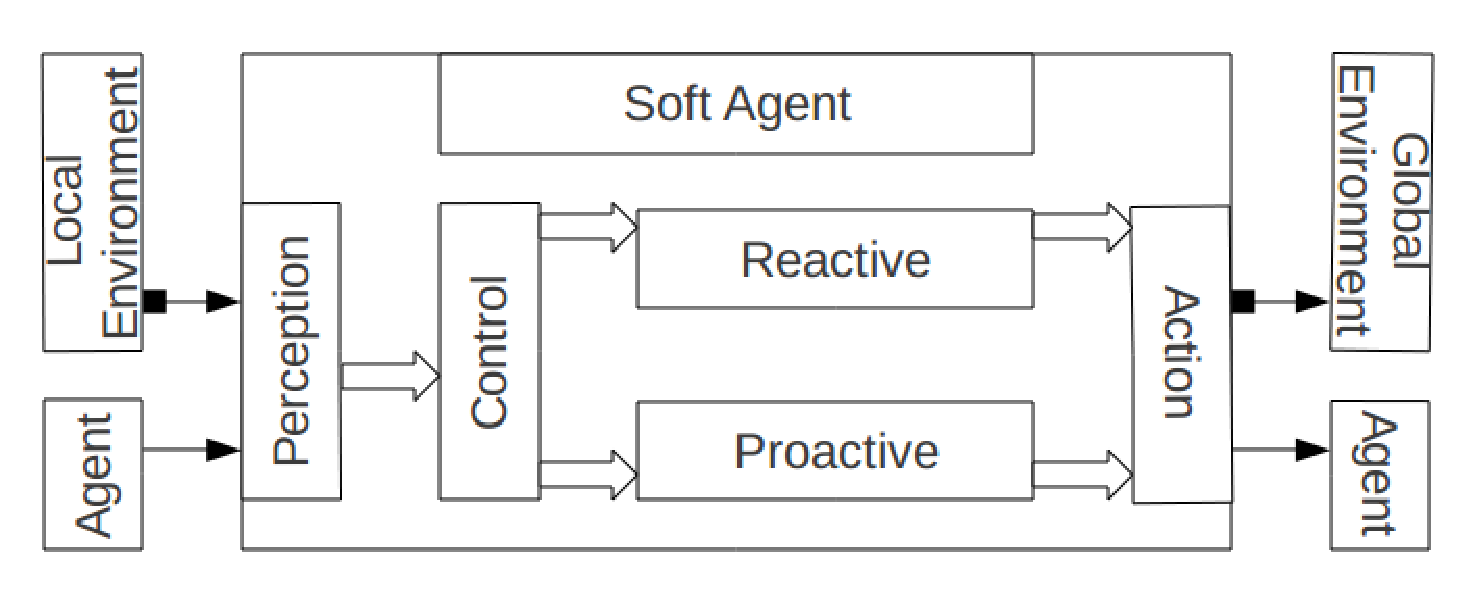
\includegraphics[width=0.5\textwidth]{softagent}
%  \caption{A soft agent senses its local environment and acts on the global environment.
%}
%  \label{fig:softagent}
%\end{figure}
\begin{figure}[h!]
\centerline{\psfig{figure=softagent.eps,width=0.75\textwidth}}
      \caption{A soft agent senses its local environment and acts on the global environment.}
\label{fig:softagent}
\end{figure}


An important property of the soft agents is that they only can sense their local environment. They can communicate with remote agents, but their vision is limited to a local neighbourhood and they maintain little information about their state. Nevertheless they can act on the global environment.  

As seen in Figure ~\ref{fig:softagent}, a soft agent perceives its local environment though the $Perception$ layer. This layer is also responsible for listening to  messages from other, possibly remote, agents. The $Controller$ layer is responsible for deciding which of the following layers should have control over the agent. The control layer can be implemented as a set of control rules which can also act as a filter suppressing information from sensors. The reactive layer provides an immediate response to changes that occur in the local environment. Roughly speaking, it implements a mapping $situation \rightarrow action$. The $Procative$ layer achieves the agent's proactive behaviour, it ensures that the agent reaches its goal. The $Action$ layer is responsible for executing the selected action on the environment (local or global) and with dispatching messages to other agents.

We will consider that the environment may be in any of the states given by:
\begin{align}
S=\{s_{1}, s_{2}, \ldots , s_{n} \}
\end{align}
Let us remark that a simplifying assumption has been made for the environment being considered discrete. But any continuous environment can be modelled by a discrete environment to any desired degree of accuracy \cite{Wooldridge09AnIntroduction}.

The set of actions an agent may choose from is given by:
\begin{align}
A=\{a_{1},a_{2}, \ldots , a_{n} \}
\end{align}

At time $t$ the environment is in some state $s_{t}$, and the agent picks an action $a_{t} \in A(s_{t})$ to be executed. As a result of this action, the agent receives a reward $r_{t+1} \in \mathbb{R}$ and the environment reaches a new state $s_{t+1}$. Given the new state, the agent chooses another action to be executed and so on.

Thus the interaction between the agent and its environment is a sequence of environment state-reward pairs and actions:
\begin{align}
h: (s_{0},r_{0}) \xrightarrow{a_{0}} (s_{1},r_{1}) \xrightarrow{a_{1}} \ldots \xrightarrow{a_{u-1}} (s_{u},r_{u})
\end{align}

In order to represent the effect of an agent's actions over the environment, the following a state transformer function is considered:
\begin{align}
env:S \times \mathbb{R} \times A \rightarrow \powerset (S \times \mathbb{R})
\end{align}

According to this definition environments are assumed to be history dependent. This means that the next state of an environment is determined by the action chosen by the agent given the current state, the reward and also by the earlier actions made by the agent. This behaviour is thus non-deterministic. In other words, the result of performing an action given a state is uncertain.

So the environment may be formally written as a triple $Env= \langle S, (s_{0}, r_{0}), env \rangle,$ where $S$ represent the set of all possible states of the environment, $s_{0}$ is the starting state, $r_{0}$ is the initial reward and $env$ is the state transformer function.

We introduce the abstract soft agent model which as a function which assigns actions to sequences of state-reward pairs:
\begin{align}
agent: (S \times \re)^{*} \rightarrow A
\end{align}
So, roughly speaking, a soft agent chooses its next action based on its previous experience, i.e., previous environment states. 

If $agent: (S \times \re)^{*} \rightarrow A$ is an agent, $env:S \times \mathbb{R} \times A \rightarrow \powerset (S \times \mathbb{R})$ is an environment, $s_{0}$ is the initial state and $r_{0}$ is the initial reward then the sequence:
\begin{align}
h: (s_{0},r_{0}) \xrightarrow{a_{0}} (s_{1},r_{1}) \xrightarrow{a_{1}} \ldots \xrightarrow{a_{u-1}} (s_{u},r_{u})
\end{align}
is a possible history of the given agent in the given environment if and only if the following conditions hold:
\begin{enumerate}
\item
$\forall u \in \nat, a_{u}=agent(((s_{0},r_{0}),(s_{1},r_{1}),\ldots ,(s_{u},r_{u})))$
\item
$\forall u \in \nat \; such \; that \; u > 0, (s_{u},r_{u}) \in env(s_{u-1}, r_{u-1},a_{u-1})$
\end{enumerate}
The set of all such possible histories will be denoted with $H$.

Now that we defined the abstract agent model we may go further in describing the main function of each of its layers as shown in Figure ~\ref{fig:softagent}.

The $Perception$ layer has two main input channels: one for the information received from the local environment and the other for the messages received from other agents. The function $see$ will map environment states to percepts and the function $listen$ will map messages received from other agents to percepts. Let us denote with $Per$ the set of percepts and with $M$ the set of messages and then the functions $see$ and $listen$ are:
\begin{align}
see: S \rightarrow Per
\label{fn:see}
\end{align}
\begin{align}
listen: M \rightarrow Per
\end{align}

The perceptions are sent further to the $Control$ layer which is responsible for deciding which is the layer that should take control over the agent --- the $Reactive$ layer or the $Proactive$ layer. The $Control$ layer could also be used as a filter for sensory information. This layer may be implemented as a set of control rules like:
\begin{align}
if \; perception \;  instanceof(M) \;  then  \; activate \; proactive \; layer
\end{align}
The rules could be updated at runtime through messages from other agents or from a supervising authority ensuring thus an adaptive behaviour of the activation layers. 

The $Reactive$ layer is responsible for handling sensory data received from the local environment. From a highly abstract point of view, the $Reactive$ layer could be seen as an agent with states \cite{Wooldridge09AnIntroduction}, like in Figure ~\ref{fig:agentstate}
%\begin{figure}[h!]
%  \centering
%  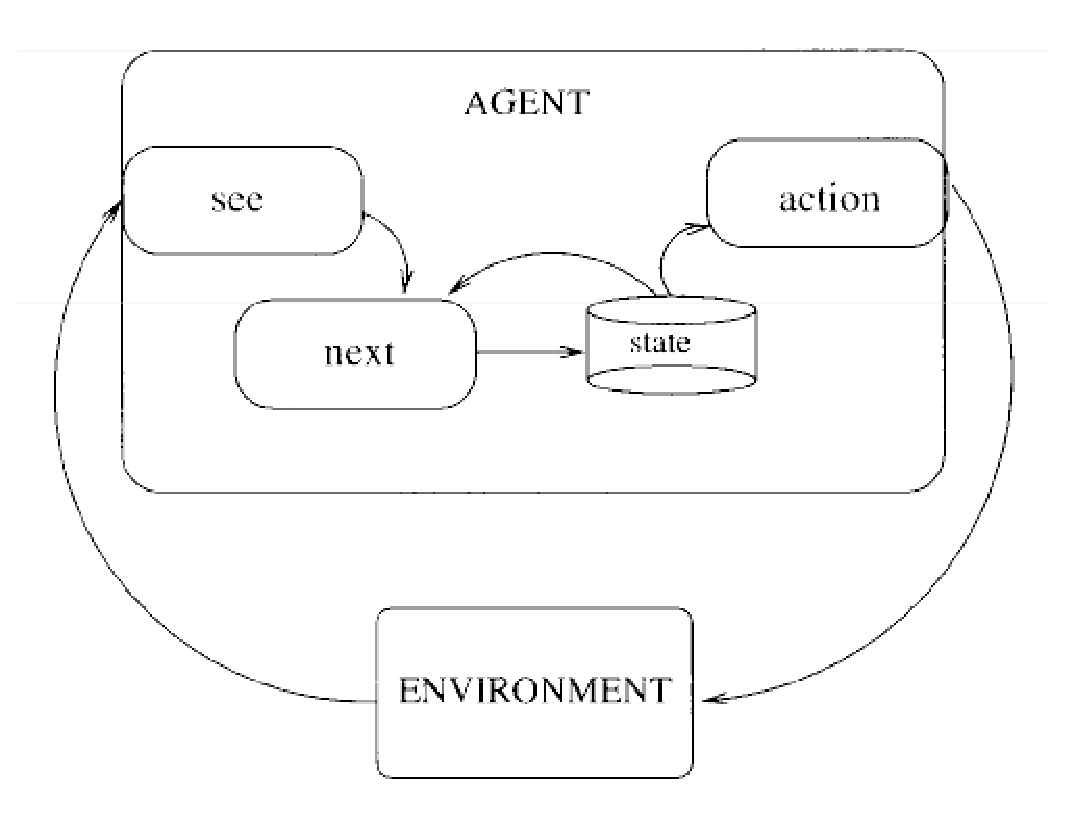
\includegraphics[width=0.5\textwidth]{agentstate}
%  \caption{A state agent.
%}
%  \label{fig:agentstate}
%\end{figure}
\begin{figure}[h!]
\centerline{\psfig{figure=agentstate.eps,width=0.5\textwidth}}
      \caption[A state agent.]{A state agent. Image source:  \cite{Wooldridge09AnIntroduction}.}
\label{fig:agentstate}
\end{figure}


The $see$ function from Figure \ref{fig:agentstate} is the one defined in relation (\ref{fn:see}).
The action-selection function is:
\begin{align}
action : I \rightarrow A,
\end{align}
where $I$ be the set of all internal states of the agent.
The function $next$ 
\begin{align}
next: I \times Per \rightarrow I.
\end{align}
is a mapping from internal states and percepts to internal states.

The behaviour of a state-based agent can be summarized as follows \cite{Wooldridge09AnIntroduction}. The agent starts in some initial internal state $i_{0}$; it then observes its environment state $s$, and generates a percept $see(s)$. The internal state of the agent is then updated via the $next$ function, becoming set to $next(i_{0}, see(s))$. The action selected by the agent is then $action(next(i_{0}, see(s))$. This action is then performed, and the agent enters another cycle, perceiving the world via $see$, updating its state via $next$, and choosing an action to perform via $action$. 

In the soft agent case the $next$ function may be replaced by a fuzzy inference system \cite{Guillaume10Interpretable}. The process of fuzzy inference implies formulating a mapping from a given input to an output using fuzzy logic elements like membership functions, logical operators, fuzzy IF-THEN rules \cite{website:fuzzyinference}.
 
Fuzzy inference systems have been successfully applied in fields such as automatic control, data classification, decision analysis, expert systems, and computer vision. Because of its multidisciplinary nature, fuzzy inference systems are associated with a number of names, such as fuzzy-rule-based systems, fuzzy expert systems, fuzzy modelling, fuzzy associative memory, fuzzy logic controllers, and simply (and ambiguously) fuzzy systems \cite{website:fuzzyinference}.

In the following the fuzzy inference process will be explained though an example of the two input, one output, three rule tipping problem taken from \cite{website:fuzzyinference}. The basic tipping problem is the following: given a number between $0$ and $10$ that represents the quality of service at a restaurant (where 10 is excellent), what should the tip be?

The example uses a process which is slightly different from Mamdani's fuzzy inference method \cite{Mamdani75AnExperiment} --- among the first control systems built using fuzzy set theory where intended to control a steam engine and boiler combination by synthesizing a set of linguistic control rules obtained from experienced human operators. \cite{website:fuzzyinference}. 

The basic structure of the example is shown is Figure ~\ref{fig:tipping}.
%\begin{figure}[h!]
%  \centering
%  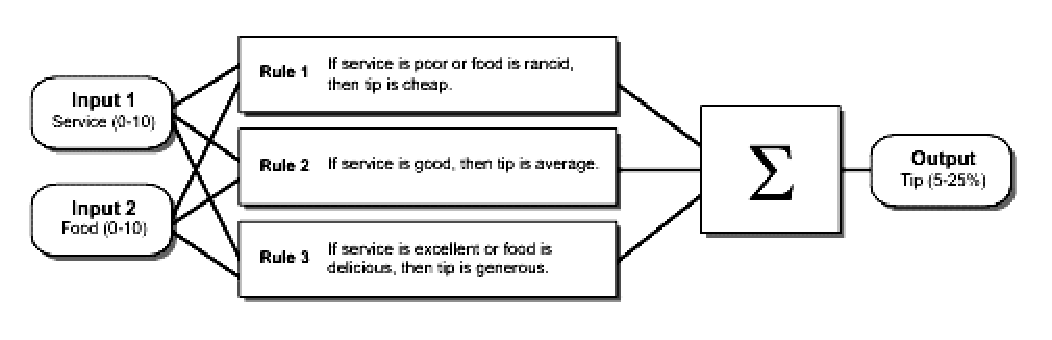
\includegraphics[width=0.75\textwidth]{tipping}
%  \caption{Dinner for two. Two inputs, one output, three rules.
%}
%  \label{fig:tipping}
%\end{figure}
\begin{figure}[h!]
\centerline{\psfig{figure=tipping.eps,width=0.75\textwidth}}
      \caption[Example --- tipping problem.]{Dinner for two. Two inputs, one output, three rules. Image source: \cite{website:fuzzyinference}.}
\label{fig:tipping}
\end{figure}


Information flows from left to right, from two inputs to a single output. The parallel nature of the rules is one of the more important aspects of fuzzy logic systems. Instead of sharp switching between modes based on breakpoints, logic flows smoothly from regions where the system's behaviour is dominated by either one rule or another.

The fuzzy inference process takes place in the following steps: fuzzification of the input variables, application of the fuzzy operator (AND or OR) in the antecedent, implication from the antecedent to the consequent, aggregation of the consequents across the rules and defuzzification. The process will be briefly described bellow, step by step.

The first step is to take the inputs and determine the degree to which they belong to each of the appropriate fuzzy sets via membership functions. After the inputs are fuzzified, one knows the degree to which each part of the antecedent is satisfied for each rule. If the antecedent of a given rule has more than one part, the fuzzy operator is applied to obtain one number that represents the result of the antecedent for that rule. Every rule may have a weight (a number between $0$ and $1$), which is applied to the number given by the antecedent. Generally, this weight is $1$ (as it is for this example) and thus has no effect at all on the implication process. After proper weighting has been assigned to each rule, the implication method is implemented. A consequent is a fuzzy set represented by a membership function, which weights appropriately the linguistic characteristics that are attributed to it. The input for the implication process is a single number given by the antecedent, and the output is a fuzzy set. The process described so far (taken from \cite{website:fuzzyinference}) can be viewed in Figure ~\ref{fig:fuzzyimplication}.
%\begin{figure}[h!]
%  \centering
%  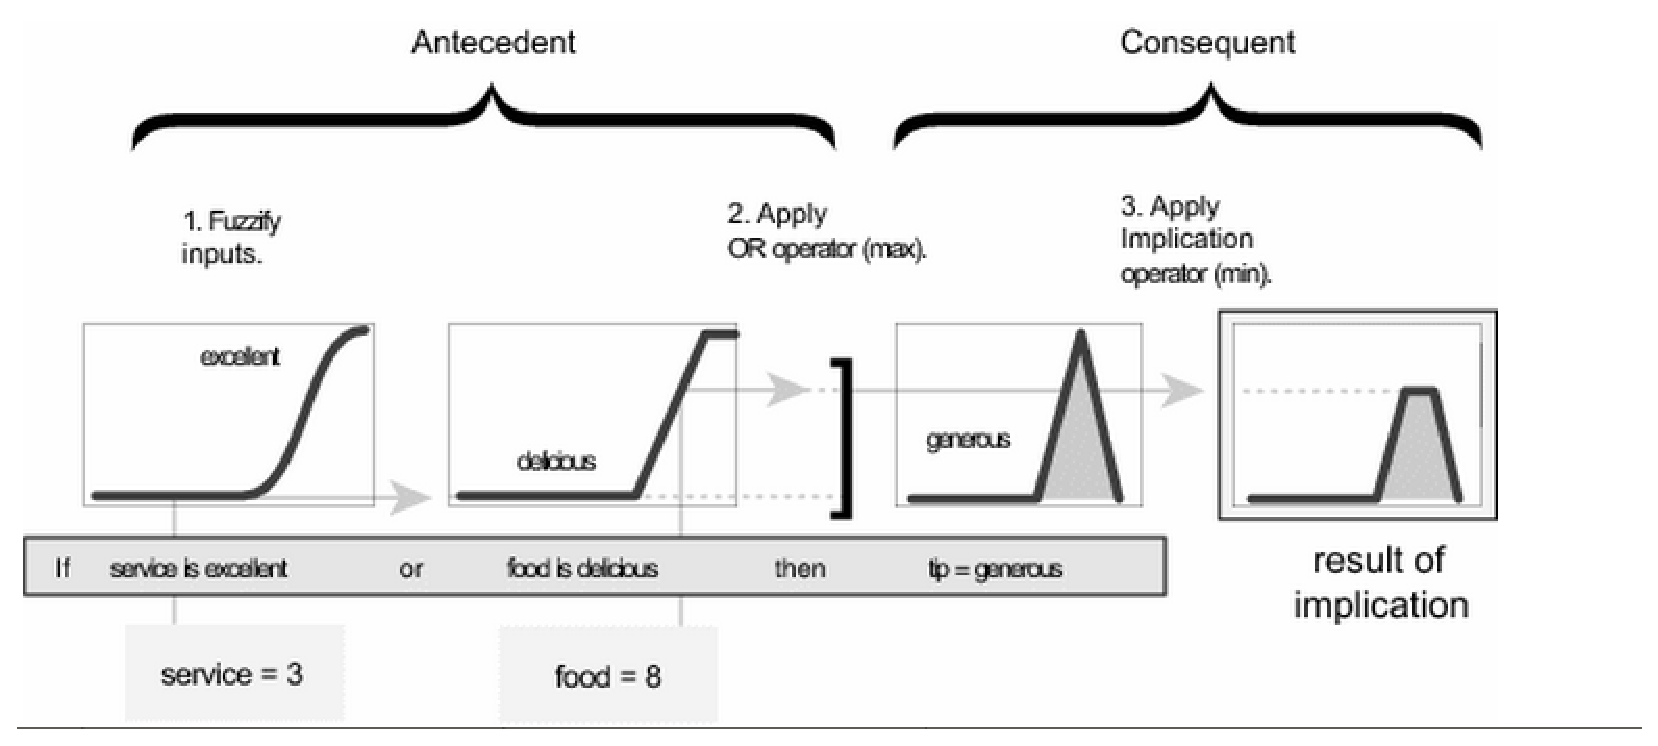
\includegraphics[width=0.75\textwidth]{fuzzyimplication}
%  \caption{The first input is $service=3$ and the second input is $food=8$. The result of the implication process is a %fuzzy set.
%}
%  \label{fig:fuzzyimplication}
%\end{figure}
\begin{figure}[h!]
\centerline{\psfig{figure=fuzzyimplication.eps,width=0.75\textwidth}}
      \caption[Fuzzy inference example.]{The first input is $service=3$ and the second input is $food=8$. The result of the implication process is a fuzzy set. Image source: \cite{website:fuzzyinference}. }
\label{fig:fuzzyimplication}
\end{figure}

Because decisions are based on the testing of all of the rules in a FIS, the rules must be combined in some manner in order to make a decision. Aggregation is the process by which the fuzzy sets that represent the outputs of each rule are combined into a single fuzzy set. Aggregation only occurs once for each output variable, just prior to the fifth and final step, defuzzification. The input of the aggregation process is the list of truncated output functions returned by the implication process for each rule. The output of the aggregation process is one fuzzy set for each output variable. So the input for the defuzzification process is a fuzzy set (the aggregate output fuzzy set) and the output is a single number. Perhaps the most popular defuzzification method is the centroid calculation, which returns the center of area under the curve \cite{website:fuzzyinference}. The entire inference process is best described by Figure ~\ref{fig:fuzzyinference}.
%\begin{figure}[h!]
%  \centering
%  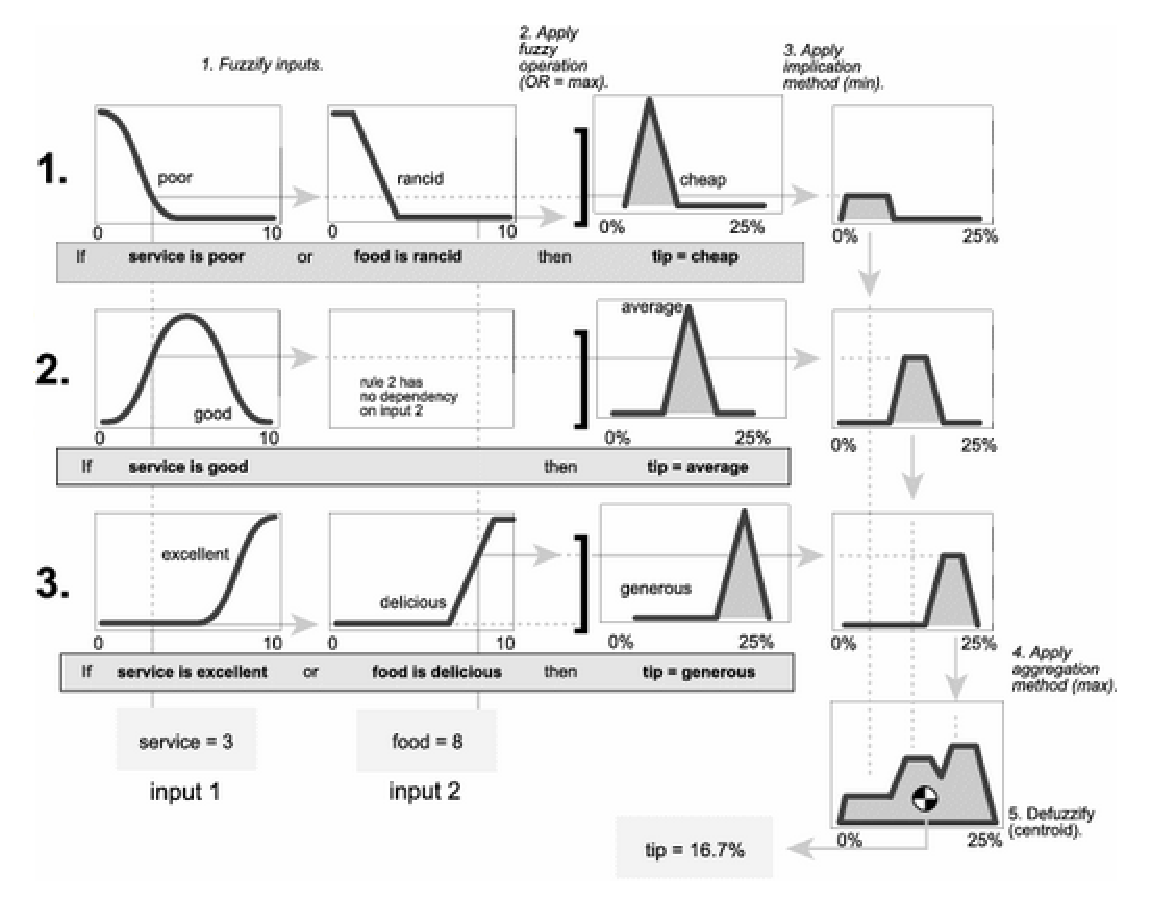
\includegraphics[width=0.9\textwidth]{fuzzyinference}
%  \caption{The fuzzy inference process.
%}
%  \label{fig:fuzzyinference}
%\end{figure}
\begin{figure}[h!]
\centerline{\psfig{figure=fuzzyinference.eps,width=0.75\textwidth}}
      \caption[Fuzzy inference process.]{The fuzzy inference process. Image source:  \cite{website:fuzzyinference}.}
\label{fig:fuzzyinference}
\end{figure}


While the $Reactive$ layer is responsible for the actions done by the agent as a response to changes in the local environment, the $Proactive$ layer is the one that ensures us that the agent does what is suppose to do. And now the question is how to specify the task that the agent has to carry out. Since writing a program to be executed by the agent is out of question because there may be some unforeseen situations in which only an agent could be able to respond accordingly. It may do so if we told him what to do instead of telling him how to do a certain task. Agents are told what to do in an indirect manner, through a performance measure. In the case of soft agents fitness functions are associated to states of the environment and the agent has to maximize its fitness. The fitness function is defined in the following way:
\begin{align}
F: H \rightarrow \re ,
\end{align}
where $H$ is the set of histories. So a fitness function associates a real value to every history.

The task that an agent has to accomplish is to maximize its fitness so an optimum is then reached for:
\begin{align}
\argmax_{agent} \sum_{h \in H(agent, Env)} F(h) P (h | agent, Env),
\end{align}
where $P (h | agent, Env)$ denotes the probability that the history $h$ occurs when the $agent$ is placed in environment $Env$.

While the fitness function evaluates what is good on a long term, the reward function evaluates the quality of a certain state. So the reward function shows which would be the good and the bad actions to be taken from a certain state. The reward function could be used to modify an agent's policy $\pi$, i.e, the agent's behaviour. Thus the reward function is defined as
\begin{align}
Q: S \times A \rightarrow \re
\end{align}
and maps a real value, a reward, to a state-action pair.

\subsection{Possible extensions and applications}

By bypassing the reactive layer and sending state-reward pairs to the $Proactive$ layer the soft agent may be used as a reinforcement learning agent as discussed in Section \ref{sec:rl}. Applications in Multi-objective optimization problems are discussed in Section \ref{sec:moop}.


\subsubsection{Reinforcement learning}
\label{sec:rl}

Reinforcement learning is a formal computational model inspired by the way in which animals acquire complex behaviour: they learn to obtain rewards and to avoid punishments. A learning agent repeatedly observes the state of its environment and then chooses which actions to perform. Performing an action changes the state of the environment and the agent receives a numeric reward. The agent must learn how to choose actions in order to maximize the total reward on a long term. There are two main approaches for this: 
\begin{itemize}
\item
	learning the utility function
	\item
	learning the reward (action-value) function
\end{itemize}

We will focus on the second approach, that is, learning the reward function. This is also known as Q-learning \cite{Watkins89Learning}.

A soft agent has a reward function $Q:S \times A \rightarrow \re$. This function is part of the $Proactive$ layer.  In order to deal with a purely reinforcement learning agent, the $Control$ layer should be programmed to only send the state-reward pairs to the $Proactive$ layer and not to the $Reactive$ layer.

Each time the state has changes new values are calculated for each combination of a state $s \in S$, and action $a \in A$ so the the algorithm basically consists in the following update:
\begin{align}
Q(s_{t},a_{t}) \leftarrow Q(s_{t},a_{t}) (1-\alpha(s_{t},a_{t})) + \alpha(s_{t},a_{t}) [ R(s_{t+1}) + \gamma \max_{a_{t+1}} Q(s_{t+1},a_{t+1})  ],
\end{align}
where $R(s_{t+1})$ is the reward observed from $s_{t}$, $\alpha(s_{t},a_{t})$ is the learning rate and $0 \leq \gamma < 1$ is the discount factor.
A learning rate equal to $0$ will make the agent not learn anything, while a learning rate equal to $1$ would make the agent consider only the most recent information. A discount factor equal to $0$ will make the agent ``opportunistic'' by considering only current rewards. The convergence of the algorithm was presented by Watkins and Dayan \cite{Watkins92Technical}.

\subsubsection{Multi-objective optimization}
\label{sec:moop}

When an optimization problem involves more than one objective function, the task of finding one (or more) optimum
solution(s), is known as the Multi-Objective Optimization Problem (MOOP). In problems characterized by more than one conflicting objective, there is no single optimum solution; instead there exists a set of solutions which are all optimal, called the Optimal Pareto front. A general multi-objective optimization problem is defined as follows (minimization case) \cite{Narzisi06Multiobjective}:
\begin{align}
\begin{array}{ll}
min & O(x)=[o_{1}(x), o_{2}(x), \ldots , o_{M}(x)] \\
subject \; to & E(x)=[e_{1}(x), e_{2}(x), \ldots , e_{L}(x)] \geq 0 \\
& x_{i}^{(L)} \leq x_{i} \leq x_{i}^{(U)} , i=1 \ldots N,
\end{array}
\end{align}
where $x=(x_{1},x_{2}, \ldots , x_{N})$ is an array of $N$ decision variables, $M$ is the number of objectives $o_{i}$,  $L$ is the number of constraints $e_{j}$ and $x_{i}^{(L)}$ and $x_{i}^{(U)}$ are respectively the lower and upper bound for each decision variable $x_{i}$. Two different solutions are compared using the concept of dominance, which induces a strict partial order in the objective space $O$. Here a solution $a$ is said to dominate a solution $b$ if it is better or equal in all objectives and better in at least one objective . For the minimization case we have \cite{Narzisi06Multiobjective}:
\begin{align}
O(a) \prec O(b) \; iff \; \left\{
\begin{array}{ll}
o_{i}(a) \leq o_{i}(b) & \forall i \in 1, \ldots , M \\
\exists j \in 1, \ldots , M & o_j(a) < o_{j}(b)
	\end{array}
\right.
\end{align}

In many situations it is actually the case that multi-objective problems need to deal with two conflicting objectives: maximizing profit and minimizing the cost of a product, maximizing performance and minimizing fuel consumption of a vehicle and so on. A soft agent could be employed for solving a two-objective optimization problem in the following way: one objective could be assigned to the $Reactive$ layer and the other one to the $Proactive$ layer. Actually an agent's behaviour is optimal if it finds a right balance between its two stances: reactive and pro-active. So the task of the agent is to minimize the function $O(x)=[o_{1}(x), o_{2}(x)]$ where $o1$ is the function performed by the $Reactive$ layer and $o2$ is the fitness function of the $Proactive$ layer. 
For multiple objectives more agents could be launched.


\section{A new approach to the set covering problem}
\label{sec:scp}

The set covering problem is a classical problem in computer science and complexity theory and it serves as a model for many real-world applications especially in the resource allocation area. In an environment where the demands that need to be covered change over time, special methods are needed that adapt to such changes. We reformulate the set covering problem as a clustering problem where the within cluster sum of squared errors to be minimized corresponds to the cost associated to a certain set covering that needs to be minimal. We have developed an incremental clustering algorithm in order to address the set covering problem. The algorithm continuously considers new items to be clustered. Whenever a new data item arrives it is encapsulated by an agent which will autonomously decide to be included in a certain cluster in the attempt to either maximize its cover or minimize the cost. We have introduced the soft agent model in order to encapsulate this behaviour. Initial tests suggest the potential of our approach.


\subsection{SCP overview}

The Set Covering Problem (SCP) is a classical problem in computer science and complexity theory and it serves as a model for many applications in the real world like: facility location problem, airline crew scheduling, resource allocation, assembly line balancing, vehicle routing, information retrieval etc. Let us consider a set $X$ and a family $F$ of subsets of $X$ such that every element from $X$ belongs to at least one subset from $F$. The set covering problem is the problem of finding a minimum number of subsets from $F$ (or subsets of minimum cost) such that their union is the set $X$.

The set covering problem is NP-hard and it has been addressed in many ways over time \cite{Gouwanda08Evolutionary, 	Crawford11AHybrid, Catalano01Parallel,Beasley96AGenetic,Alon03OnlineSCP,Alfandari10ClusteredSCP}. A straightforward solution is the greedy approximation algorithm \cite{Cormen09Introduction}. This method selects at each step a set from $F$ that covers most of the still uncovered elements.
In \cite{Beasley96AGenetic} the set covering problem is addressed using a genetic algorithm by using an $n$-bit binary string as the chromosome structure, where $n$ is the number of columns from the SCP dataset. In order to mark that column $i$ is in the solution the $i^{th}$ is set to $1$. The authors designed heuristic operators that transform invalid solutions (obtained after applying genetic operators) to valid ones. The binary tournament
selection was chosen as the method for parent selection and for crossover the authors propose a so-called  fusion operator taking into account both the structure and the relative fitnesses of the parents. A variable mutation rate specified in \cite{Beasley96AGenetic} is used arguing that the genetic algorithm is more effective. Computational experiments on a large set of randomly generated problems show that the genetic algorithm based approach is capable of producing high quality solutions. 
In \cite{Alon03OnlineSCP} the online version of SCP is considered. In the online version an adversary gives elements to the algorithm from one by one. Whenever a new element is arriving, the algorithm has to cover it.  The elements of $X$ and the members of $F$ are known in advance to the algorithm, but the set $X^{'} \subseteq X$ of
elements given by the adversary isn't and the task is to minimize the total cost of the sets chosen by the algorithm. 
In \cite{Crawford11AHybrid} the set covering problem is addressed using an ant colony optimization algorithm together with a new transition rule. The authors have also used a look-ahead mechanism for constraint consistency checking such that new elements are added to the solution if they do not produce conflicts with the next element to be chosen.
In \cite{Alfandari10ClusteredSCP} a clustered variant of the SCP is defined. In the Clustered-SCP the subsets are partitioned into $k$ clusters and a fixed cost is associated to each cluster. So the objective is to find a cover that minimizes the sum of subsets costs plus the sum of fixed cluster costs.

The classical set covering problem can be formulated as a clustering problem where the within cluster sum of squared errors to be minimized corresponds to the cost associated to a certain set covering that needs to be minimal. We have developed an incremental clustering algorithm in order to address the set covering problem. The algorithm continuously considers new items to be clustered. Whenever a new data item arrives it is encapsulated by an agent which will autonomously decide to be included in a certain cluster in the attempt to either maximize its cover or minimize the cost. 

In machine learning, clustering is an example of unsupervised learning because it does not rely on predefined classes and class-labelled training examples. So it could be said that clustering is a form of learning by observation, as opposed of being a form of learning by examples. In data analysis, efforts have been conducted on finding efficient  cluster analysis methods for  large datasets. The main requirements for a good clustering algorithm would be the scalability of the method, its effectiveness in clustering complex data shapes and types, dealing with high-dimensional data, and handling mixed data, i.e.,  both numerical and categorical data.

There is a great variety of clustering algorithms to choose from each with its own strengths and weaknesses. In \cite{Gaceanu11AnIncremental} an incremental clustering algorithm is presented. Incremental clustering algorithms in general do not rely on the in-memory dataset and they build the solution gradually, with every new incoming data item. The idea behind is that it is possible to consider one instance at a time and assign it to existing clusters without significantly affecting the already existing structures. Only the cluster representations need to be kept in memory so not the entire dataset and thus the space requirements for such an algorithm are very small. Whenever a new instance is considered an incremental clustering algorithm would basically try to assign it to one of the already exiting clusters. Such a process is not very complex and therefore the time requirements for an incremental clustering algorithm are also small.

Let us consider a set $X$ and a family of subsets of $X$ 
\begin{align}
F= S_{1}, S_{2}, \dots , S_{n}.
\end{align}
The classical set covering problem is the problem of finding a minimum cardinality $J \subseteq {1, \dots, n}$ such that
\begin{align}
\cup_{j \in J} S_{j} = X.
\end{align}

The set covering problem is NP-hard \cite{Cormen09Introduction} and it can be approached by the following greedy approximation algorithm:
\begin{algorithm}
\caption{SCP-Greedy}
\label{alg:SCP-Greedy}
\begin{algorithmic}[1]
\STATE $U \leftarrow X$
\STATE $C \leftarrow \emptyset$
\WHILE {$U \neq \emptyset$}
\STATE find $S_{j}$ such that $\mid S_{j} \cap U \mid $ is maximal, where $j \in J$
\STATE $U \leftarrow U - S_{j}$
\STATE $C \leftarrow C \cup \{S_{j}\}$
\ENDWHILE
\end{algorithmic}
\end{algorithm}

The algorithm iteratively selects the set $S_{j}$ which covers the most still uncovered elements from $X$. The set $U$ contains the still uncovered elements and at the beginning it is equal to $X$. At each step the algorithm is choosing a set $S_{j}$ that covers most of the elements that are left uncovered up to this point. The set $S_{j}$ is added to $C$ and in the end $C$ will contain a subfamily of sets that cover $X$. The algorithm finishes when $U$ is empty.

The minimum cost set covering problem considers a cost $c_{j}$ for each $S_{j}$ and the problem is to find a cover for $X$ and to minimize the sum of costs $\sum_{j \in J} c_{j}$.

\subsection{Incremental SCP}
\label{sec:proposed}


In our model the input is an $m \times n$ incidence matrix $A$, where $m=\mid X \mid$ and each column corresponds to a set $S_{j}$ with $j \in \{1, \dots , n \}$. Each column $j$ has a corresponding cost $c_j > 0$. We say that a column $j$ covers a row $i$ if $a_{ij}=1$. Let $x_j$ be a binary decision variable which has the value $1$ if column $j$ is chosen and $0$ otherwise. Then the set covering problem can be defined as minimize (\ref{rel:cost}) subject to (\ref{rel:cover}) \cite{Crawford11AHybrid}.

\begin{align}
\label{rel:cost}
f(x)=\sum_{j=1}^{n}{c_{j}x_{j}},
\end{align}

\begin{align}
\label{rel:cover}
\sum_{j=1}^{n}{a_{ij}x_{j}} \geq 1, \forall i=\overline{1,n},
\end{align}

\begin{align}
x_{j} = \left\{
    \begin{array}{ll}
        1, & if~ column~ $j$~ is~ chosen\\
        0, & otherwise.
    \end{array}
\right.
\end{align}

%
%\begin{align}
%x_{j} = \left\{
%	\begin{array}{ll}
%	1 & if ~column ~j ~is ~chosen\\
%	0 & otherwise
%	\end{array}
%	\right.
%\end{align}

Clustering can be seen as the problem of finding ''meaningful'' groups in data and a way to do this is by minimizing a certain objective function. 
The set covering problem can be formulated as a clustering problem in the following way: assign columns from $A$ to clusters such that the function from (\ref{rel:cost}) is minimized and the cluster is valid, i.e., the relation (\ref{rel:cover}) holds.

We have developed an incremental clustering algorithm in order to address the set covering problem. The algorithm considers one instance at a time and assigns it to one of the existing clusters without significantly affecting the already existing structures. The algorithm continuously considers new items to be clustered. Whenever a new data item arrives it is encapsulated by an agent which will autonomously decide to join a certain cluster in the attempt to either maximize the cluster cover or minimize its the cost. These two objectives are rather conflicting and this brings a great deal of imprecision and uncertainty in the whole reasoning process. That is why we have employed \emph{soft agents} in this matter. A \emph{soft agent} is an intelligent agent that has to deal with imprecision, uncertainty, partial truth and approximation during its execution as a reactive agent or goal oriented agent or both as explained in Section \ref{subsec:softagentmodel}.

For the set covering problem we define the fitness of an agent $a_{i}$ given a cluster $c_{k}$ in the following way:

\begin{definition}
The fitness of an agent $a_{i}$ given a cluster $c_{k}$ is:
\begin{align}
f(a_{i}, c_{k}) = \frac{\mid rows(a_{i}) - rows(c_{k}) \mid}{m},
\end{align}
where:
\begin{itemize}
\item $rows(a_{i})$ denotes the set of rows covered by agent $a_{i}$,
\item $rows(c_{k})$ denotes set of rows covered by cluster $c_{k}$,
\item $m$ is the total number of rows.
\end{itemize} 
\end{definition}

The algorithm considers one column at a time and encapsulates it in a agent. In the first part an initial valid cluster will be built using a greedy approach (a cluster is valid if it covers the considered set). After this step every newly considered agent will decide weather to try to maximize the cover of one of the existing clusters or to minimize the cost using the following control function: $f^{\lambda}(a_{i},c_{k})$. The parameter $\lambda$ is increasing in time thus leading to agents that act upon minimizing the cost rather than maximize the cover.
A pseudo-code of the algorithm is sketched in Algorithm \ref{alg:incremental_SCP}.


\begin{algorithm}
\caption{Incremental SCP}
\label{alg:incremental_SCP}
\begin{algorithmic}[1]
\STATE initialize parameters
\STATE find a proper cluster $c_{0}$ by randomly selecting agents
\STATE $C \leftarrow C \cup \{c_{0}\}$
\WHILE {$condition()$}
\STATE $U \leftarrow U \cup \{createAgent()\}$ 
\WHILE {$U \neq \emptyset $}
\IF {$reactive(a_{i}) $}
\STATE assign $a_{i}$ to a non-valid cluster $c_{k}$ or create a new cluster 
\ELSE
\STATE $\{S_{j}, c_{k}\} \leftarrow tryReplace(a_{i})$
\STATE $U \leftarrow U \cup S_{j}$
\ENDIF
\ENDWHILE
\STATE $U \leftarrow U \cup discardWorseCluster()$
\STATE update parameters
\ENDWHILE
\end{algorithmic}
\end{algorithm}


The algorithm continuously receives new items (columns) to be clustered and an agent encapsulates each item. The agent is placed in the collection $U$ of unclustered items. Starting from line $6$ the algorithm repetitively considers agents from the collection $U$. The agent decides to behave in a reactive or proactive manner based on its control function. If it decides to behave reactively, i.e., maximize the cover then the agent attempts to find a non-valid cluster to be included in. If no such cluster is found then a new cluster is created containing this agent. The new cluster is added to $C$ and $a_{i}$ is removed from $U$. A cluster is valid if all the rows are covered (\ref{rel:cover}). If on the other hand the agent wants to minimize the cost then   
it will try to replace agents from a valid cluster $c_{k}$. If the replace operation took place then the set of replaced agents $S_{j}$ is added to the unclustered collection. After all agents from $U$ have been added to some clusters the cluster with the worse cost is discarded and its agents are added to the unclustered collection. Parameters like $\lambda$ or acceptable cost threshold may be updated at this point. The whole process starts over from line $4$ and ends when some condition is met (like a good-enough solution is found or a certain number of iterations have been completed). 


Initial tests have been done on the $scp410$ dataset from the $OR-Library$ \cite{website:scp} which is a collection of test data sets for a variety of operation research (OR) problems, including SCP. The $scp410$ dataset has $200$ rows and $1000$ columns in the following format: number of rows ($m$), number of columns ($n$), the cost of each column $c(j),j=1,\dots,n$ and then for each row $i (i=1,\dots,m)$: the number of columns which cover row $i$ followed by a list of the columns which cover row $i$.

We have obtained near-optimum solutions as shown in Figure \ref{fig:scp410fig1}. Reference \cite{Crawford11AHybrid} mentions that the optimum cost is $514$. After $15000$ iterations we have obtained the cost $561$. By one iteration we mean the execution of the loop from $line~4$ of Algorithm \ref{alg:incremental_SCP}. At each iteration we read one new agent until all agents have been read. The $scp410$ dataset may produce at most $1000$ agents. At iteration $1000$ we have already obtained the cost $774$ so at the beginning the algorithm finds good solutions fast. Unfortunately, in time, it slows down. We are confident that a careful analysis of the implementation will lead to a decrease in the running time. Tests on other datasets from \cite{website:scp} are ongoing.

\begin{figure}[h!]
\centerline{\psfig{figure=scp410fig1.eps,width=0.75\textwidth}}
      \caption{Execusion on scp410. }
\label{fig:scp410fig1}
\end{figure}


We have developed an incremental clustering algorithm in order to address the set covering problem. The algorithm continuously considers new items to be clustered. Whenever a new data item arrives it is encapsulated by an agent which will autonomously decide to join a certain cluster in the attempt to either maximize the cluster cover or minimize its the cost. We have used soft agents in order to deal with the two conflicting objectives: maximize cover and minimize cost. As in any approximation algorithm an optimal solution is not guaranteed to be found, the purpose being to find reasonably good solutions fast enough. Ongoing tests on large datasets \cite{website:scp} suggest promising results and lead us to also consider similar problems like the set partitioning problem.

\section{Conclusions and future work}
\label{sec:scpconcfw}

In this chapter we have presented our contributions to NP optimization problems namely to the travelling salesman problem and to the set covering problem. These approaches have been presented in our original papers \cite{Chira07Stigmergic, Gaceanu12SCP}.

We have seen that the proposed SAS approach for solving TSP is a powerful optimization technique that combines the advantages of two models: Ant Colony Systems and Multi-Agent Systems. Interoperation between agents is based on both indirect communication --- given by pheromone levels --- and direct knowledge sharing, greatly reducing the risk of
falling into the trap of local minima. Experimental results on standard datasets outline the advantage of the approach over the classical Ant Colony Systems.
We have also developed an incremental clustering algorithm in order to address the set covering problem. The algorithm continuously considers new items to be clustered. Whenever a new data item arrives it is encapsulated by an agent which will autonomously decide to join a certain cluster in the attempt to either maximize the cluster cover or minimize its the cost. We have used soft agents in order to deal with the two conflicting objectives: maximize cover and minimize cost. As in any approximation algorithm an optimal solution is not guaranteed to be found, the purpose being to find reasonably good solutions fast enough. Ongoing tests on large datasets \cite{website:scp} suggest promising results.

For each original approach proposed in this chapter we have emphasized improvement possibilities and possible future extensions.

As future research directions we intend to improve the approaches presented in this chapter, to extend the evaluation of the proposed techniques and to investigate  and develop other computational models for addressing NP-hard problems.


Ongoing research focuses on numerical experiments to demonstrate the robustness of the proposed model. The SAS method has to be further refined in terms of types of messages that agents can directly exchange. Furthermore, other metaheuristics are investigated with the aim of identifying additional potentially beneficial
hybrid models.
